\documentclass[11pt]{article}

%% PACKAGES
\usepackage{graphicx}
\usepackage[printonlyused]{acronym}
\usepackage{float}
\usepackage[colorlinks=false]{hyperref}
\usepackage{tabularx}
\usepackage{caption}
\usepackage[margin=1.0in]{geometry}
\usepackage{tocloft}
\usepackage{listings}

\lstset{basicstyle=\small\ttfamily,columns=flexible,breaklines=true,xleftmargin=0.5in,keepspaces=true}

\setcounter{tocdepth}{3}
\setcounter{secnumdepth}{3}

\makeatletter
\g@addto@macro\normalsize{%
  \setlength\abovedisplayskip{0.25pt}
  \setlength\belowdisplayskip{0.25pt}
  \setlength\abovedisplayshortskip{0.25pt}
  \setlength\belowdisplayshortskip{0.25pt}
}
\makeatother

\setlength{\parskip}{\baselineskip}

%% GRAPHICS PATH
\graphicspath{{../../../shared_latex_inputs/images}{../../../shared_latex_inputs/graphs}}

\newcommand{\acposs}[1]{%
	\expandafter\ifx\csname AC@#1\endcsname\AC@used
	\acs{#1}'s%
	\else
	\aclu{#1}'s (\acs{#1}'s)%
	\fi
}

\title{\Huge EMTG Tutorial: \\ Propagation and Force Models}
\vspace{0.5cm}
\author
{
	Tim Sullivan \thanks{Aerospace Engineer, The Aerospace Corporation}
}
\vspace{0.5cm}

\newcommand{\listofknownissuesname}{\Large List of Known Issues}
\newlistof{knownissues}{mcf}{\listofknownissuesname}

\newcommand{\knownissue}[3]
{
	\refstepcounter{knownissues}
	\par\noindent\textbf{\hyperref[#2_b]{\theknownissues\quad #1}}\label{#2_h}
	\textbf{\hfill\pageref{#2_b}}
	#3
}

\newcommand{\knownissuelabel}[2]
{
	 \phantomsection
  	\hyperref[#2_h]{#1}\def\@currentlabel{\unexpanded{#1}}\label{#2_b}
}

\begin{document}

\begin{titlepage}
\maketitle
\thispagestyle{empty}
\begin{table}[H]
	\centering
	\begin{tabularx}{\textwidth}{|l|l|X|}
		\hline
		\textbf{Revision Date} & \textbf{Author} & \textbf{Description of Change} \\
		\hline
		\date{December 2, 2022} & Tim Sullivan & Initial revision.\\
		\hline
		\date{June 30, 2023} & Joseph Hauerstein & Conversion to \LaTeX.\\ 
		\hline
		\date{August 4, 2023} & Joseph Hauerstein & Addition of Known Issues section.\\ 
		\hline
	\end{tabularx}
\end{table}
\end{titlepage}

\newpage
\tableofcontents
\thispagestyle{empty}
\newpage

\listofknownissues
\thispagestyle{empty}

\knownissue{The ``rk7813M adaptive step'' integrator does not work}{broken_integrator_issue}

\newpage
\clearpage
\setcounter{page}{1}



%\section*{List of Acronyms}
\begin{acronym}
%To define the acronym and include it in the list of acronyms: \acro{acronym}{definition}
%To define the acronym and exclude it from the list of acronyms:  \acro{acronym}{definition}
%
%\ac{acronym} Expand and identify the acronym the first time; use only the acronym thereafter
%\acf{acronym} Use the full name of the acronym.
%\acs{acronym} Use the acronym, even before the first corresponding \ac command
%\acl{acronym}  Expand the acronym without using the acronym itself.
%
%

\acro{TCM}{trajectory correction maneuver}
\acro{ACO}{Ant Colony Optimization}
\acro{AD}{Automatic Differentiation}
\acro{ADL}{Architecture Design Laboratory}
\acro{ADM}{asteroid departure maneuver}
\acro{AEI}{atmospheric entry interface}
\acro{AES}{Advanced Exploration Systems}
\acro{AGA}{aerogravity assist}
\acro{ALARA}{As Low As Reasonably Achievable}
\acro{API}{application programming interface}
\acro{BB}{branch and bound}
\acro{BVP}{Boundary Value Problem}
\acro{CATO}{Computer Algorithm for Trajectory Optimization}
\acro{CL}{confidence level}
\acro{CONOPS}{concept of operations}
\acro{COV}{Calculus of Variations}
\acro{D/AV}{Descent/Ascent Vehicle}
\acro{DE}{Differential Evolution}
\acro{RLA}{Right Ascension of Launch Asymptote}
\acro{DLA}{Declination of Launch Asymptote}
\acro{DPTRAJ/ODP}{Double Precision Trajectory and Orbit Determination Program}
\acro{DSH}{Deep Space Habitat}
\acro{DSN}{Deep Space Network}
\acro{DSMPGA}{Dynamic-Size Multiple Population Genetic Algorithm}
\acro{EB}{Evolutionary Branching}
\acro{ECLSS}{environmental control and life support system}
\acro{EGA}{Earth gravity assist}
\acro{ELV}{expendable launch vehicle}
\acro{EMME}{Earth to Mars, Mars to Earth}
\acro{EMMVE}{Earth to Mars, Mars to Venus to Earth}
\acro{EMTG}{Evolutionary Mission Trajectory Generator}
\acro{EVMME}{Earth to Venus to Mars, Mars to Earth}
\acro{EVMMVE}{Earth to Venus to Mars, Mars to Venus to Earth}
\acro{ERRV}{Earth Return Re-entry Vehicle}
\acro{FISO}{Future In-Space Operations}
\acro{FMT}{Fast Mars Transfer}
\acro{GASP}{Gravity Assist Space Pruning}
\acro{GCR}{galactic cosmic radiation}
\acro{GRASP}{Greedy Randomized Adaptive Search Procedure}
\acro{GSFC}{Goddard Space Flight Center}
\acro{GTOC}{Global Trajectory Optimization Competition}
\acro{GTOP}{Global Trajectory Optimization Problem}
\acro{HAT}{Human Architecture Team}
\acro{HGGA}{Hidden Genes Genetic Algorithm}
\acro{IMLEO}{Initial Mass in \acl{LEO}}
\acro{IPOPT}{Interior Point OPTimizer}
\acro{ISS}{International Space Station}
\acro{JHUAPL}{Johns Hopkins University Applied Physics Laboratory}
\acro{JSC}{Johnson Space Center}
\acro{KKT}{Karush-Kuhn-Tucker}
\acro{LEO}{Low Earth Orbit}
\acro{LRTS}{lazy race tree search}
\acro{MAT}{Mars Architecture Team}
\acro{MONTE}{Mission analysis, Operations, and Navigation Toolkit Environment}
\acro{MCTS}{Monte Carlo tree search}
\acro{MGA}{Multiple Gravity Assist}
\acro{MIRAGE}{Multiple Interferometric Ranging Analysis using GPS Ensemble}
\acro{MOGA}{Multi-Objective Genetic Algorithm}
\acro{MOSES}{Multiple Orbit Satellite Encounter Software}
\acro{MPI}{message passing interface}
\acro{MPLM}{Multi-Purpose Logistics Module}
\acro{MSFC}{Marshall Space Flight Center}
\acro{NELLS}{NASA Exhaustive Lambert Lattice Search}
\acro{NMDB}{Navigation and Mission Design Branch}
\acro{NSGA}{Non-Dominated Sorting Genetic Algorithm}
\acro{NSGA-II}{Non-Dominated Sorting Genetic Algorithm II}
\acro{NHATS}{Near-Earth Object Human Space Flight Accessible Targets Study}
\acro{NTP}{Nuclear Thermal Propulsion}
\acro{OD}{orbit determination}
\acro{OOS}{On-Orbit Staging}
\acro{PCC}{Pork Chop Contour}
\acro{PEL}{permissible exposure limits}
\acro{PLATO}{PLAnetary Trajectory Optimization}
\acro{REID}{risk of exposure-induced death}
\acro{RTBP}{Restricted Three Body Problem}
\acro{SA}{Simulated Annealing}
\acro{SLS}{Space Launch System}
\acro{SNOPT}{Sparse Nonlinear OPTimizer}
\acro{SOI}{sphere of influence}
\acro{SPE}{solar particle events}
\acro{SQP}{sequential quadratic programming}
\acro{SRAG}{Space Radiation Analysis Group}
\acro{TEI}{Trans-Earth Injection}
\acro{TIM}{technical interchange meeting}
\acro{TOF}{time of flight}
\acro{TPBVP}{Two Point Boundary Value Problem}
\acro{TMI}{Trans-Mars Injection}
\acro{VARITOP}{Variational calculus Trajectory Optimization Program}
\acro{VGA}{Venus gravity assist}
\acro{VILM}{v-infinity leveraging maneuver}
\acro{MOI}{Mar Orbit Injection}
\acro{PCM}{Pressurized Cargo Module}
\acro{STS}{Space Transportation System}
\acro{EDS}{Earth Departure Stage}
\acro{NEO}{near-Earth asteroid}
\acro{IDC}{Integrated Design Center}
\acro{SEP}{solar-electric propulsion}
\acro{SRP}{solar radiation pressure}
\acro{NEP}{nuclear-electric propulsion}
\acro{REP}{radioisotope-electric propulsion}
\acro{DRM}{Design Reference Missions}

\acro{ASCII}{American Standard Code for Information Interchange}
\acro{AU}{Astronomical Unit}
\acro{BWG}{Beam Waveguides}
\acro{CCB}{Configuration Control Board}
\acro{CMO}{Configuration Management Office}
\acro{CODATA}{Committee on Data for Science and Technology}
\acro{DEEVE}{Dynamically Equivalent Equal Volume Ellipsoid}
\acro{DRA}{Design Reference Asteroid}
\acro{EME2000}{Earth Centered, Earth Mean Equator and Equinox of J2000 (Coordinate Frame)}
\acro{EOP}{Earth Orientation Parameters}
\acro{ET}{Ephemeris Time}
\acro{FDS}{Flight Dynamics System}
\acro{FTP}{File Transfer Protocol}
\acro{GSFC}{Goddard Space Flight Center}
\acro{PI}{Principal Investigator}
\acro{HEF}{High Efficiency}
\acro{IAG}{International Association of Geodesy}
\acro{IAU}{International Astronomical Union}
\acro{IERS}{International Earth Rotation and Reference Systems Service}
\acro{ICRF}{International Celestial Reference Frame}
\acro{ITRF}{International Terrestrial Reference System}
\acro{IOM}{Interoffice Memorandum}
\acro{JD}{Julian Date}
\acro{JPL}{Jet Propulsion Laboratory}
\acro{LM}{Lockheed Martin}
%\acro{LP150Q}{}
%\acros{LP100K}{}
\acro{MAVEN}{Mars Atmosphere and Volatile EvolutioN}
\acro{MJD}{Modified Julian Date}
\acro{MOID}{Minimum Orbit Intersection Distance}
\acro{MPC}{Minor Planet Center}
\acro{NASA}{National Aeronautics and Space Administration}
\acro{NDOSL}{\ac{NASA} Directory of Station Locations}
\acro{NEA}{near-Earth asteroid}
\acro{NEO}{near-Earth object}
\acro{NIO}{Nav IO}
\acro{OSIRIS-REx}{Origins, Spectral Interpretation, Resource Identification, and Security-Regolith Explorer}
\acro{PHA}{Potentially Hazardous Asteroid}
\acro{PHO}{Potentially Hazardous Object}
\acro{SBDB}{Small-Body Database}
\acro{SI}{International System of Units}
\acro{SPICE}{Spacecraft Planet Instrument Camera-matrix Events}
\acro{SPK}{SPICE Kernel}
\acro{SRC}{Sample Return Capsule}
\acro{SSD}{Solar System Dynamics}
\acro{AGI}{Analytical Graphics, Inc.}
\acro{STK}{Systems Tool Kit}
\acro{TAI}{International Atomic Time}
\acro{TBD}{To Be Determined}
\acro{TBR}{To Be Reviewed}
\acro{TCB}{Barycentric Coordinate Time}
\acro{TDB}{Temps Dynamiques Barycentrique, Barycentric Dynamical Time}
\acro{TDT}{Terrestrial Dynamical Time}
\acro{TT}{Terrestrial Time}
\acro{URL}{Uniform Resource Locator}
\acro{UT}{Universal Time}
\acro{UT1}{Universal Time Corrected for Polar Motion}
\acro{UTC}{Coordinated Universal Time}
\acro{USNO}{U. S. Naval Observatory}
\acro{YORP}{Yarkovsky-O'Keefe-Radzievskii-Paddack}

\acro{NLP}{nonlinear program}
\acro{MBH}{monotonic basin hopping}
\acro{MBH-C}{monotonic basin hopping with Cauchy hops}
\acro{FBS}{forward-backward shooting}
\acro{MGALT}{Multiple Gravity Assist with Low-Thrust}
\acro{MGALTS}{Multiple Gravity Assist with Low-Thrust using the Sundman transformation}
\acro{MGA-1DSM}{Multiple Gravity Assist with One Deep Space Maneuver}
\acro{MGAnDSMs}{Multiple Gravity Assist with $n$ Deep-Space Maneuvers using Shooting}
\acro{PSFB}{Parallel Shooting with Finite-Burn}
\acro{PSBI}{Parallel Shooting with Bounded Impulses}
\acro{FBLT}{Finite-Burn Low-Thrust}
\acro{FBLTS}{Finite-Burn Low-Thrust using the Sundman transformation}
\acro{ESA}{European Space Agency}
\acro{ACT}{Advanced Concepts Team}
\acro{IRAD}{independent research and development}
\acro{Isp}[$\text{I}_{sp}$]{specific impulse}
\acro{GA}{genetic algorithm}
\acro{GALLOP}{ Gravity Assisted Low-thrust Local Optimization Program}
\acro{MALTO}{Mission Analysis Low-Thrust Optimization}
\acro{PaGMO}{Parallel Global Multiobjective Optimizer}
\acro{FRA}{feasible region analysis}
\acro{CP}{conditional penalty}
\acro{HOC}{hybrid optimal control}
\acro{HOCP}{hybrid optimal control problem}
\acro{PSO}{particle swarm optimization}
\acro{SEPTOP}{Solar Electric Propulsion Trajectory Optimization Program}
\acro{STOUR}{Satellite Tour Design Program}
\acro{STOUR-LTGA}{Satellite Tour Design Program - Low Thrust, Gravity Assist}
\acro{PaGMO}{Parallel Global Multiobjective Optimizer}
\acro{SDC}{static/dynamic control}
\acro{DDP}{Differential Dynamic Programming}
\acro{HDDP}{Hybrid Differential Dynamic Programming}
\acro{ACT}{Advanced Concepts Team}
\acro{GMAT}{General Mission Analysis Toolkit}
\acro{BOL}{beginning of life}
\acro{EOL}{end of life}
\acro{KSC}{Kennedy Space Center}
\acro{VSI}{variable \ac{Isp}}
\acro{RTG}{radioisotope thermal generator}
\acro{ASRG}{advanced Stirling radiosotope generator}
\acro{ARRM}{Asteroid Robotic Redirect Mission}
\acro{AATS}{Alternative Architecture Trade Study}
\acro{PPU}{power processing unit}
\acro{STM}{state transition matrix}
\acro{MTM}{maneuver transition matrix}
\acro{BCI}{body-centered inertial}
\acro{BCF}{body-centered fixed}
\acro{UTTR}{Utah Test and Training Range}
\acro{EPV}{equatorial projection of $\mathbf{v}_\infty$}
\acro{KBO}{Kuiper belt object}
\acro{DSM}{deep-space maneuver}
\acro{BPT}{body-probe-thrust}
\acro{4PL}{four parameter logistic}
\acro{BCF}{body-centered fixed}

\acro{SPT}{Sun-probe-thrust}
\acro{PIRATE}{PVDrive Interface and Robust Astrodynamic Target Engine}
\acro{PEATSA}{Python EMTG Automated Trade Study Application}
\acro{NEXT}{NASA's Evolutionary Xenon Thruster}
\acro{TAG}{Touch and Go}
\acro{KBO}{Kuiper Belt object}

\acro{CDR}{critical design review}
\acro{PDR}{preliminary design review}
\acro{CCAFS}{Cape Canaveral Air Force Station}

\acro{MRD}{Mission Requirements Document}
\acro{EDL}{entry, descent, and landing}

\acro{Earth-GRAM}{Earth Global Reference Atmospheric Model}
\acro{POST II}{Program to Optimize Simulated Trajectories II}
\acro{MONSTER}{Monte-Carlo Operational Navigation Simulation for Trajectory Evaluation and Research}

\acro{ZSOI}{zero sphere of influence}
\end{acronym}

% --------------------------------------------------------------------------------------------------------------------------
% --------------------------------------------------------------------------------------------------------------------------


%%%%%%%%%%%%%%%%%%%%%
\section{Introduction}
\label{sec:introduction}
%%%%%%%%%%%%%%%%%%%%%

Previous tutorials did not account for forces beyond the point-mass gravity of the central body. In this tutorial, you’re going to update a few of the previous \ac{EMTG} options files to account for additional forces.

%%%%%%%%%%%%%%%%%%%%%
\section{Propagation in EMTG}
\label{sec:propagation_in_emtg}
%%%%%%%%%%%%%%%%%%%%%

\ac{EMTG} has two main methods for performing propagation of the spacecraft: Kepler and Integrator. Kepler uses Kepler’s equation to analytically propagate the spacecraft’s orbit state between delta-v events. The ``Integrator time step size option'' does not matter for Kepler propagation since it is analytical. Kepler propagation is compatible with \ac{MGALT}, Coast Phase, and \ac{MGAnDSMs}. (It is also compatible with the more advanced phase types \ac{PSBI} and Probe Entry Phase, which have not been covered in the tutorials yet.)

\noindent \ac{EMTG}’s Integrator option propagates the spacecraft by integrating the full equations of motion, whether they are simple two-body equations or more complex N-body equations with additional perturbations. As a result, Integrator propagation is slower than Kepler propagation but can model more realistic forces. Integrator is compatible with \ac{FBLT}, Coast Phase, and \ac{MGAnDSMs}. (It is also compatible with the more advanced phase types \ac{PSFB}, Probe Entry Phase, and Control Law Thrust Phase, which have been covered in the tutorials yet.) 

\noindent \knownissuelabel{Note: The “rk7813M adaptive step” option does not work.}{broken_integrator_issue}

\noindent The propagation type can be selected for the whole mission in the ``Physics Options'' tab or set on a Journey-by-Journey basis in the ``Journey Options'' tab by selecting ``Override journey’s propagator type?'' As the options text indicates, setting the propagator type on the ``Journey Options'' tab overrides the ``Physics Options'' selection for that particular journey as is shown in Figure \ref{fig:propagator_type_selection}. The ``Integrator time step size option'' can also be overridden on a per-Journey basis from the ``Journey Options'' tab, as well.

\begin{figure}
	\centering
	\fbox{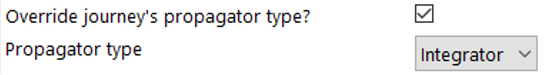
\includegraphics[width=0.7\linewidth]{Propogation_and_Force_Models_journey_options_propagator_type_selection.png}}
	\caption{\label{fig:propagator_type_selection}Journey Options Propagator Type Selection.}
\end{figure}


%%%%%%%%%%%%%%%%%%%%%
\section{Perturbation Modeling in EMTG}
\label{sec:perturbation_modeling_in_emtg}
%%%%%%%%%%%%%%%%%%%%%

Through the ``Physics Options'' tab, \ac{EMTG} can model perturbing forces due to \ac{SRP}, gravitational forces other than those from the central body known as third-body or n-body forces, forces due to the oblateness of the central body with the J2 zonal coefficient, spherical harmonics gravity, and atmospheric drag. Spherical harmonics and drag require additional input files and are beyond the scope of this tutorial.

\noindent Perturbation effects (i.e., non-two-body forces) are modeled in different ways depending on the ``Mission Type'' or transcription method selected in either the ``Global Mission Options'' (or ``Journey Options'' tab when using variable ``Mission Types''). Perturbations are modeled differently or may not be available depending on the ``Mission Type'' in use. Table \ref{tab:prop_and_preturb_options} shows a summary of compatible perturbations and ``Mission Types''. This section will go over the differences for the major transcription methods you’ve used so far and more detail on how they model perturbations.

\begin{table}[H]
	\begin{small}
		\begin{tabularx}{\linewidth} { >{\arraybackslash} X >{\arraybackslash} X >{\arraybackslash} X}
			\hline
			Mission Type & Propagation & Perturbation Modeling \\
			\hline 
			Coast Phase & Integrator or Kepler & Only with Integrator \\ 
			\ac{MGAnDSMs} & Integrator or Kepler & Only with Integrator \\ 
			\ac{MGALT} & Kepler & Yes \\
			\ac{FBLT} & Integrator & Yes \\
 			\hline
		\end{tabularx}
	\end{small}
	\caption{\label{tab:prop_and_preturb_options}Journey Options Propagator Type Selection.}
\end{table}

%%%%%%%%%%%%%%%%%%%%%
\subsection{MGALT}
\label{sec:mgalt}
%%%%%%%%%%%%%%%%%%%%%

\acf{MGALT} models each Journey using the Sims-Flanagan transcription and Kepler propagation. A bounded-impulse delta-v is applied at each segment to model the spacecraft’s thrust; the magnitude of the impulse is limited to the maximum delta-v that could be achieved by thrusting constantly across the segment. If any perturbations are turned on, they are applied in a similar manner: the perturbing force(s) are evaluated at the point at which each propulsive delta-v is applied. The effect of the perturbing acceleration(s) across the segment is approximated by multiplying the acceleration by the time between segments. The perturbing ``delta-v'' is then added to the propulsive delta-v to get the full impulse applied to the spacecraft. As a result, \ac{MGALT} can approximate the effect of perturbing accelerations without using Integrator propagation. Figure \ref{fig:mgalt_mission_type} shows a diagram of the \ac{MGALT} model.

\begin{figure}[H]
	\centering
	\fbox{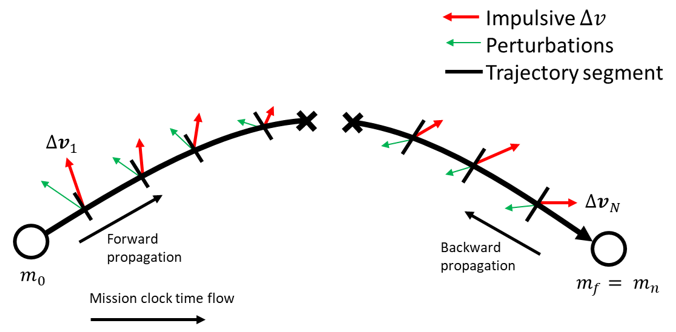
\includegraphics[width=\linewidth]{Propogation_and_Force_Models_mgalt_mission_type.png}}
	\caption{\label{fig:mgalt_mission_type}\ac{MGALT} Mission Type.}
\end{figure}

%%%%%%%%%%%%%%%%%%%%%
\subsection{FBLT}
\label{sec:fblt}
%%%%%%%%%%%%%%%%%%%%%

\acf{FBLT} is similar to \ac{MGALT} except numerical integration is used to propagate the equations of motion for the spacecraft rather than Sims-Flanagan transcription. The central body, thrust, and perturbing forces sum to apply a net acceleration to the spacecraft, which is integrated with a Runge-Kutta method to generate the spacecraft trajectory. This gives a more realistic trajectory than \ac{MGALT}. A diagram of the \ac{FBLT} model is shown in Figure \ref{fig:fblt_mission_type}.

\begin{figure}
	\centering
	\fbox{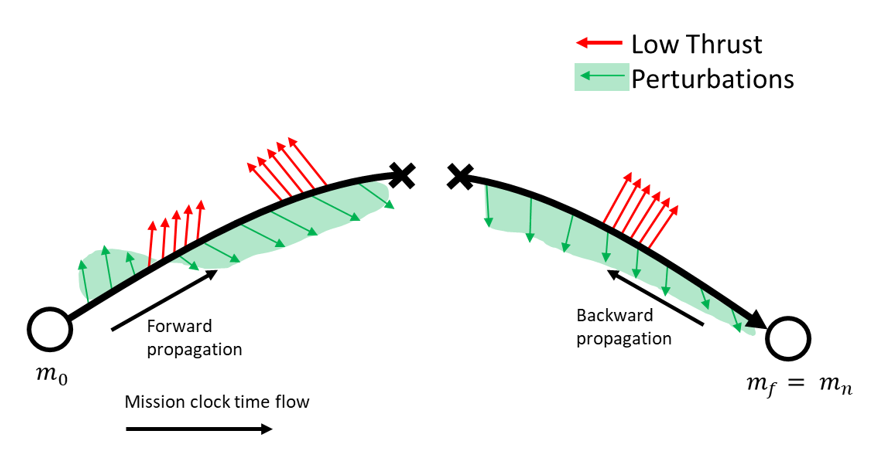
\includegraphics[width=\linewidth]{Propogation_and_Force_Models_fblt_mission_type.png}}
	\caption{\label{fig:fblt_mission_type}\ac{FBLT} Mission Type.}
\end{figure}

%%%%%%%%%%%%%%%%%%%%%
\subsection{MGAnDSMs}
\label{sec:mgandsms}
%%%%%%%%%%%%%%%%%%%%%

\acf{MGAnDSMs} allows for some user-selectable number of impulsive maneuvers during each Journey. Spacecraft propagation can be modeled with Kepler or Integrator between instantaneous delta-v events at each \ac{DSM}. Perturbations can only be applied with Integrator propagation by adding the perturbing forces to the central body gravitational force. Figure \ref{fig:mgandsms_mission_type} shows a diagram of the \ac{MGAnDSMs} model.

\begin{figure}[H]
	\centering
	\fbox{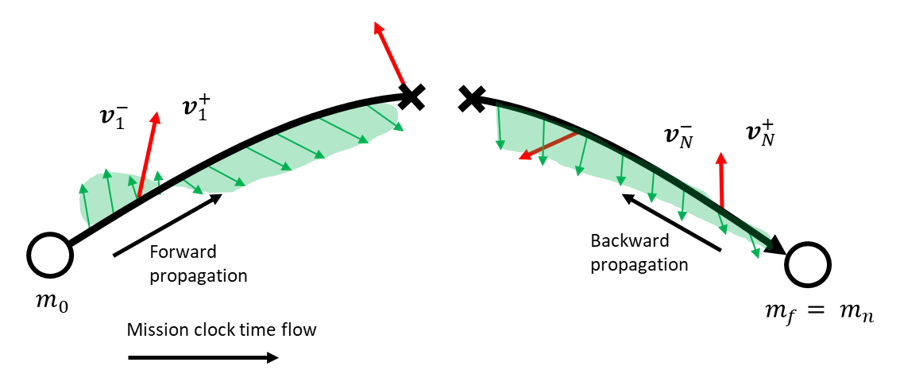
\includegraphics[width=\linewidth]{Propogation_and_Force_Models_mgansdsms_mission_type.png}}
	\caption{\label{fig:mgandsms_mission_type}\ac{MGAnDSMs} Mission Type. Integrator propagation is required to model perturbations.}
\end{figure}

%%%%%%%%%%%%%%%%%%%%%
\subsection{Coast Phase}
\label{sec:coast_phase}
%%%%%%%%%%%%%%%%%%%%%

Like the name implies, Coast Phase has no spacecraft thrust. It can be propagated with either Kepler (and no perturbing forces) or Integrator with optional perturbing forces. For a Coast Phase, the ``Integrator time step size'' set on the ``Physics Options'' tab is always overridden by the forward/backward half-phase step size values on the ``Journey Options'' tab.

%%%%%%%%%%%%%%%%%%%%%
\section{Tutorial Problem Setup}
\label{sec:tutorial_problem_setup}
%%%%%%%%%%%%%%%%%%%%%

Begin by making a copy of the LowSIRIS-REx tutorial working directory. Call the new directory \texttt{Force\_Models}. Create a results directory in \texttt{Force\_Models}. Open the LowSIRIS-REx.emtgopt file with PyEMTG. Update the path to the Universe folder in the ``Physics Options'' tab if you are not using a Universe folder that is shared between multiple tutorials. Update the hardware library path in the ``Spacecraft Options'' tab (don’t forget the trailing slash). Switch to the ``Output Options'' tab and select the ``Override working directory?'' check box. Change the path to \texttt{Force\_Models/results}. Save the .emtgopt file in \texttt{Force\_Models}, keeping the same filename.

%%%%%%%%%%%%%%%%%%%%%
\subsection{Initial Run}
\label{sec:initial_run}
%%%%%%%%%%%%%%%%%%%%%

Run the LowSIRIS-REx \ac{EMTG} options file (File -\textgreater run, or Ctrl+r). You will compare the solutions you generate with additional forces modeled to this two-body, \ac{MGALT} solution. After executing the first run, with the \ac{EMTG} options file still open in PyEMTG, switch to the ``Global Options'' tab and rename the file to \texttt{LowSIRIS-REx\_forcemodel}. Save the file (File -\textgreater save, or Ctrl + s).

%%%%%%%%%%%%%%%%%%%%%
\subsection{Physics Options}
\label{sec:physics_options}
%%%%%%%%%%%%%%%%%%%%%

Switch to the ``Physics Options'' tab. On the far right of PyEMTG, there is a section called ``Perturbation settings''. This section switches on common perturbing forces including \ac{SRP}, third-body effects, and central-body J2. 

%%%%%%%%%%%%%%%%%%%%%
\subsubsection{SRP}
\label{sec:srp}
%%%%%%%%%%%%%%%%%%%%%

Select ``Enable SRP''. This will reveal new parameters for the spacecraft and Sun used to configure the \ac{SRP} force model as shown in Figure \ref{fig:perturbation_settings}. The spacecraft parameters you can set are the spacecraft cross-sectional area exposed to the Sun and spacecraft coefficient of reflectivity. \ac{EMTG} models a consistent surface area exposed to the Sun and does not adjust for spacecraft attitude (i.e., the cannonball model). This should be sufficient for this stage of the mission design.

\noindent Additionally, \ac{EMTG} allows you to set values pertaining to the solar activity by changing the ``Solar percentage [0, 1]'' or ``Solar constant (flux at 1 \acs{AU})''. These can often be left to their default value but can be adjusted to examine the effects of flying the mission at high or low solar activity levels. Leave the \ac{SRP} values set to their default.

\noindent Selecting ``Enable SRP'' turns on \ac{SRP} perturbations for all Journeys whose Journey type supports perturbations.

\begin{figure}
	\centering
	\fbox{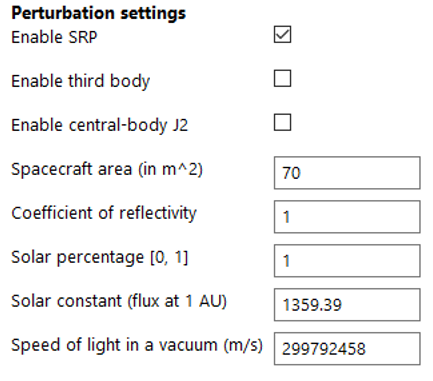
\includegraphics[width=0.5\linewidth]{Propogation_and_Force_Models_perturbation_settings.png}}
	\caption{\label{fig:perturbation_settings}Perturbation Settings.}
\end{figure}

%%%%%%%%%%%%%%%%%%%%%
\subsubsection{Third Body Forces}
\label{sec:third_body_forces}
%%%%%%%%%%%%%%%%%%%%%

Select ``Enable third body''. Checking this box reveals a new option in the ``Journey Options'' tab allowing you to select the additional gravitational bodies that will be modeled on a per-Journey basis. You will set these later.

\noindent Selecting ``Enable third body'' turns on third-body perturbations for all Journeys whose Journey type supports perturbations, but, as mentioned previously, which third bodies, if any, are perturbers is set on a per-Journey basis.

%%%%%%%%%%%%%%%%%%%%%
\subsubsection{Central-body J2}
\label{sec:central_body_j2}
%%%%%%%%%%%%%%%%%%%%%

The final perturbation option is ``Enable central-body J2''. This will switch on the J2 spherical harmonic gravitational forces for the central body of each Journey. For this force to be included, the Universe file for the central body must contain a value for J2 and a J2 reference radius (units of km) in the central body section of the Universe file. See Figure \ref{fig:mars_universe_j2} for an example of how to set these values for Mars. You won’t turn J2 perturbations on for this mission. 

\begin{figure}[H]
	\centering
	\fbox{
\includegraphics[width=0.7\linewidth]{Propogation_and_Force_Models_mars_universe_file_j2_settings.png}}
	\caption{\label{fig:mars_universe_j2}Mars Universe File J2 Settings.}
\end{figure}

\noindent Selecting ``Enable central-body J2'' turns on J2 perturbations for all Journeys whose Journey type supports perturbations.

%%%%%%%%%%%%%%%%%%%%%
\subsection{Journey Options}
\label{sec:journey_options}
%%%%%%%%%%%%%%%%%%%%%

Switch to the ``Journey Options'' tab. Notice that there is a new option toward the bottom of the window called ``Perturbation\_bodies''. You can type in the Universe file body numbers from the ``menu of bodies'' section of the central body universe file or click the ``…'' button and select the bodies you wish to include in third body effects modeling. Select Venus, Mars, Jupiter, Saturn, Uranus, and Neptune or enter ``[2,4,5,6,7,8]'' as shown in Figure \ref{fig:journey_options_perturbation_bodies}. Do not select the Earth (ID 3) because the Journey departure is an ephemeris-pegged launch or direct insertion from the Earth, meaning the departure state is coincident with the Earth. Thus, you would produce a divide-by-zero error if you attempted to calculate the gravitational force exerted by the Earth on the spacecraft at departure. Follow this procedure for both the “Earth\_to\_Bennu” Journey and the “Bennu\_to\_Earth” Journey.

\begin{figure}[H]
	\centering
	\fbox{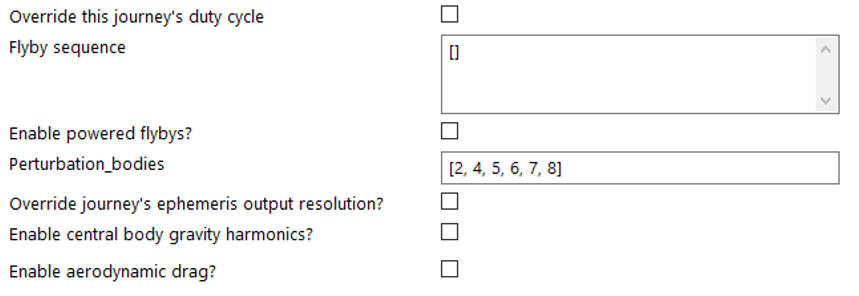
\includegraphics[width=0.9\linewidth]{Propogation_and_Force_Models_journey_options_perturbation_bodies.png}}
	\caption{\label{fig:journey_options_perturbation_bodies}Journey Options - Perturbation Bodies.}
\end{figure}

%%%%%%%%%%%%%%%%%%%%%
\subsubsection{Other Perturbing Forces}
\label{sec:other_perturbing_forces}
%%%%%%%%%%%%%%%%%%%%%

Two other types of perturbations can be turned on and off on a per-Journey basis: aerodynamic drag and central body gravity harmonics (beyond J2). The check boxes for these options are at the bottom of the ``Journey Options'' tab. Use of either of these perturbations requires an additional input file describing the coefficients used to evaluate the atmospheric density or spherical harmonics model, respectively. You will not use these perturbers in the current example, and further description is beyond the scope of this tutorial.

%%%%%%%%%%%%%%%%%%%%%
\subsection{Solver Options}
\label{sec:solver_options}
%%%%%%%%%%%%%%%%%%%%%

The easiest way to see the effects of the perturbing forces you just added is to evaluate the previous, two-body solution using this updated \ac{EMTG} options file. Switch to the ``Solver Options'' tab and change ``Inner-loop Solver Mode'' to ``Evaluate trialX''. Select the \texttt{LowSIRIS-REx.emtg} file you created earlier in this tutorial by solving the unperturbed problem as the ``Trial decision vector or initial guess'' using the ``…'' button.

%%%%%%%%%%%%%%%%%%%%%
\section{Run}
\label{sec:run}
%%%%%%%%%%%%%%%%%%%%%

%%%%%%%%%%%%%%%%%%%%%
\subsection{Evaluate Trial X}
\label{sec:evaluate_trial_x}
%%%%%%%%%%%%%%%%%%%%%

Run this mission (File -\textgreater run, or Ctrl+r) and open the resulting \ac{EMTG} file in a text editor. Notice that the results file is called \texttt{FAILURE\_LowSIRIS-REx\_forcemodel\_Sun(EB)\_Sun(BE).emtg}. Near the bottom of the file, you can see that the decision vector you used as an initial guess does not produce a feasible solution now that the force model is different. Below the objective function and worst constraint section, you should see:

\begin{lstlisting}
Number of solution attempts: 1
Solution attempt that produced a feasible solution with the best objective 
value (0 if no feasible solutions): 0
\end{lstlisting}

\noindent Look at the final state of Journey 0 (Earth to Bennu) of the \texttt{LowSIRIS-REx\_forcemodel} solution compared to the final state of the LowSIRIS-REx trial solution. They’re the same value, shouldn't this solution be feasible? Didn’t they both arrive at Bennu? The answer is no. The state you’re seeing is the same because EMTG integrates forwards \textit{and} backwards from the Journey departure and arrival states, respectively. Since you didn’t change the Bennu arrival epoch in the decision vector, you’re trying to rendezvous with Bennu at the same ephemeris point. This is the state shown in the \ac{EMTG} solution file. To see the problem, you must examine the constraint vector. This is the section at the bottom of the \ac{EMTG} solution file starting with \texttt{Fupperbounds}. The row starting with \texttt{Fdescriptions} contains the labels for each entry, and the row starting with \texttt{Constraint\_Vector} contains the scaled constraint values. You’re interested in the values for\texttt{ j\_p\_MGALT: match point} where ``j'' and ``p'' are followed by Journey and phase numbers, respectively, and the parameter after ``match point'' is the state parameter being matched. (Constraint values and bounds, as well as decision vector values and bounds, may also be viewed in a more user-friendly format in the \texttt{XFfile.csv} produced in the output directory of each \ac{EMTG} run.)

%%%%%%%%%%%%%%%%%%%%%
\subsection{NLP with Initial Guess}
\label{sec:nlp_with_initial_guess}
%%%%%%%%%%%%%%%%%%%%%

The mission needs some refinement in order to be feasible now that you have changed the force model. Luckily, the two-body solution is a good initial guess, and you only need to refine it with \acs{SNOPT}. In other words, with a good initial guess, you usually do not need \ac{MBH} to produce a feasible solution, though \ac{MBH} can still be used to try to find a more optimal trajectory. Switch to the ``Solver Options'' tab. Change the ``Inner-loop Solver Mode'' to ``\acs{NLP} with initial guess''. Rename the file \texttt{LowSIRIS-REx\_forcemodel\_nlp.emtg} in the ``Global Options'' tab and run it (File -\textgreater run, or Ctrl+r). If you are interested in watching \acs{SNOPT} iterate in real time, you can uncheck the ``Quiet \acs{NLP} solver?'' checkbox on the ``Solver Options'' tab.

\noindent Open the solution in a text editor and check that \ac{EMTG} has found a feasible solution. An example set of constraint match points for this resolved \ac{EMTG} options file is shown in the last column in Table \ref{tab:match_point_constraint_values}.

\begin{table}[H]
	\begin{small}
		\begin{tabularx}{\linewidth} { >{\arraybackslash} X >{\centering\arraybackslash} X >{\centering\arraybackslash} X >{\centering\arraybackslash} X}
			\hline
			 & Two-Body Solution & Two-Body Solution Evaluated with Perturbations & Two-Body Solution with Perturbations Resolved With \acs{SNOPT} \\
			\hline 
			j0p0MGALT: match point x\newline & -5.52E-06 & 1.27E-02 & -4.16E-06 \\ 
			j0p0MGALT: match point y\newline & -2.02E-07 & -1.63E-03 & 2.05E-07 \\ 
			j0p0MGALT: match point z\newline & 6.88E-07 & -7.01E-04 & 3.75E-07 \\
			j0p0MGALT: match point xdot\newline & -1.78E-06 & 1.10E-03 & -9.56E-07 \\
			j0p0MGALT: match point ydot\newline & -6.21E-06 & 1.11E-02 & -4.60E-06 \\
			j0p0MGALT: match point zdot & -2.67E-06 & 6.38E-03 & -2.14E-06 \\
 			\hline
		\end{tabularx}
	\end{small}
	\caption{\label{tab:match_point_constraint_values}LowSIRIS-REx Match Point Constraint Values.}
\end{table}

\noindent You can apply the same perturbations to the \ac{FBLT} LowSIRIS-REx solution. Since \ac{FBLT} integrates the full equations of motion, this will be the most accurate method for modeling the low-thrust trajectory. An important thing to keep in mind here is that an \ac{MGALT} solution can be used as an initial guess for an \ac{FBLT} problem (and vice versa) using the same ``Trial decision vector or initial guess'' option previously described. \ac{EMTG} recognizes that the initial guess decision variables are \ac{MGALT} but that the new problem is \ac{FBLT}, and internally adapts the decision variables accordingly. To add perturbations to the \ac{FBLT} LowSIRIS-REx solution, perform the same modifications to the \texttt{.emtgopt} file as to the LowSIRIS-REx\_forcemodel solution in this tutorial.

\noindent This concludes the tutorial on force modeling in \ac{EMTG}. You can now apply accurate modeling of the forces on your spacecraft during each Journey. As you’ve seen, the typical \ac{EMTG} workflow is to begin with a low-fidelity but easy-to-solve version of the mission, then progressively increase the realism before arriving at a highly realistic solution that is ready for implementation in \ac{MONTE} or another system for designing the flight-ready mission. Table \ref{tab:emtg_fidelity_progression} gives example \ac{EMTG} progressions for chemical and low-thrust missions. The next tutorials will go over how to model spacecraft hardware like thrusters and power systems and how to trade different options to find the best combination for the mission.

\begin{table}[H]
	\begin{small}
		\begin{tabularx}{\linewidth} { >{\arraybackslash} X >{\arraybackslash} X }
			\hline
			Chemical & Low Thrust \\
			\hline 
			1. \ac{MGAnDSMs} with flyby sequence & 1. \ac{MGALT} with flyby sequence with perturbing forces\newline \\ 
			2. \ac{MGAnDSMs} with single-phase\newline Journeys & 2. \ac{MGALT} with single-phase Journeys with perturbing forces\newline \\ 
			3. \ac{MGAnDSMs} with propagated flybys & 3. \ac{MGALT} with propagated flybys with perturbing forces\newline \\
			4. \ac{MGAnDSMs} with propagated flybys with perturbing forces & 4. \ac{FBLT} with propagated flybys with perturbing forces\newline \\
 			\hline
		\end{tabularx}
	\end{small}
	\caption{\label{tab:emtg_fidelity_progression}Example Low to High-Fidelity Progression. Particularly for low-thrust missions, you may need to adapt these steps for your particular use case.}
\end{table}


\end{document}